\documentclass{beamer}

\usetheme{Warsaw} %// Activate for custom appearance


% Define my settings
\definecolor{mygreen}{cmyk}{.0,.60,1,.0}
\setbeamertemplate{blocks}[rounded][shadow=false]
\addtobeamertemplate{block begin}{\pgfsetfillopacity{0.8}}{\pgfsetfillopacity{1}}
\setbeamercolor{structure}{fg=mygreen}
\setbeamercolor*{block title example}{fg=blue!50,
bg= blue!10}
\setbeamercolor*{block body example}{fg= blue,bg= blue!5}



\usepackage{color}
\newcommand{\R}{\proglang{R}}
\newcommand{\pkg}[1]{{\normalfont\fontseries{b}\selectfont #1}}
\newcommand{\Rfunction}[1]{{\texttt{#1}}} 
\newcommand{\fun}[1]{{\texttt{#1}}} 
\newcommand{\Robject}[1]{{\texttt{#1}}} 



\title[Survival and latencies]{On survival analyses of the 
timing of cognitive processes}
\author[Pablo, Javier, Manolo \& Jeff]{
\includegraphics[width=3cm]{images.jpg}\\Pablo Gomez, Javier Breithaupt,  Manuel Perea \& Jeff Rouder}
\institute[UdeV-DPU-Mizzou]{DePaul U, Universitat de Valencia, U of Missouri}
\date{EMPG2015} 


\begin{document}
\frame{\titlepage}



\section{Motivation}
{
	\frame
	{
		\frametitle{Latencies}
		\begin{itemize}
			\item Understanding the micro-structure of laboratory tasks informs us about the components of cognitive function.
			\item Several tasks utilize latencies as the main dependent variable.
			\item RTs, fixation times, naming, are examples of latency based measurements.
		\end{itemize}
	}
	
			
	\frame
	{
		\frametitle{What we do with latency measurements?}
		\begin{itemize}
			\item Often, effects are explored though null-hypothesis testing on the mean latency.
     			\item This approach might be appropriate if the goal is to obtain evidence for the existence of a phenomenon \emph{per se}.
     			\item However, it might not be as informative if we are trying to understand specifically what component of processing is affected by a manipulation.
  		\end{itemize}
	 }
	 
	
	\frame
	{
  		\frametitle{What to do...}
  		There are methods to examine latency data, and each one of them requires you to make some level of theoretical assumption.
  		\begin{enumerate}
    			\item<1-> \emph{Mean RT}. No or little theoretical commitment, but misses the distributional information; however, with clever experiments (e.g., masked priming) researcher can make assumptions about the timing and locus of effects.
    			\item<2-> \emph{Functional form analyses.} It assumes that latencies can be described by distributions with known functional forms: ex-Gaussian, Weibull, etc.
    			\item<3-> \emph{Process Models.} A process model provides with a mechanism that generates the latency data. One fits the model to the data, and  then obtains parameters.
  		\end{enumerate}
	}

	\frame
	{
  		\frametitle{Survival analyses}
		Here we explore an alternative to the three methods just mentioned:  survival analyses.
	}
			
	\frame{
	  	\frametitle{The promise of survival analyses}

			\begin{enumerate}
    			\item  It goes beyond the mean RT, as it explores the full distributions of latencies. 
    			\item  It does not make assumptions about functional form, and is not subject to misspecification.
    			\item  It does not make a theoretical commitment to a process model.
		\end{enumerate}
	}
	
		\frame{
			\frametitle{The promise of survival analyses}
			In short, it might be right on the \emph{sweet spot} of data analysis. 
		}

}



\section{Survival Analysis}
{
  	\frame
  	{
     		\frametitle{What is survival?}
		
		\begin{itemize}
			\item $S(t)=Pr(T>t)$
			\item For a given time $t$, the proportion of responses with $latency > t$ are the proportion survival time at time $t$.
			\item At $t=0$, $S(0)=1$, and at longest latency, $S(t) \to 0 $ as $t \to \infty$
    		\end{itemize}
  	}


	\frame
	{
	\frametitle{In the past...}
	\begin{itemize}
		\item There have been attempts to use survival analyses and hazard functions;  see Van Zandt (2002)
		\item ``Serious hazard function analysis  would use samples of at least a few hundred observations"
		\item Estimating the tail is specially difficult. 
	\end{itemize}
	}
	
	
	\frame
	{
	\frametitle{Let's consider a manipulation with two conditions}
	\begin{itemize}
		\item <1-> A research question: Can we learn anything about the temporal dynamics of different components of processing?
		\item <2-> Divergence point corresponds to the shortest latency value at which the a manipulation has a significant impact.
		\item <3-> Sheridan (2013); Reingold et al. (2012) for first fixation durations.
		\item <3->  1-ms time bins: the survival curve was computed separately for each condition and for each participant, and then averaged across participants.
	\end{itemize}
	}
	

	
	\frame
	{
	\frametitle{Divergence point estimation. Boot strapping method}
	\begin{itemize}
		\item <1-> On each iteration, the latencies for each participant in each condition was randomly re-sampled with replacement.
		\item <2-> Each participants' survival curves were then computed and averaged (across subjects). 
		\item <3-> Next, for each time bin $t$ the $\Delta_{t,i}$ are computed ($i^{th}$: iteration from 1 to 10,000), and then sorted.
		\item <4-> The range between the 5th and the 9,995th value becomes $CI_{\Delta(t)}$ 
		\item <5-> Divergence point between conditions:  the $t$ at which $CI_{\Delta(t)} does not include 0$ 
	\end{itemize}
	}


  	\frame
  	{
     		\frametitle{Sheridan, 2013}
		\begin{figure}[htbp] %  figure placement: here, top, bottom, or page
    			\centering
    			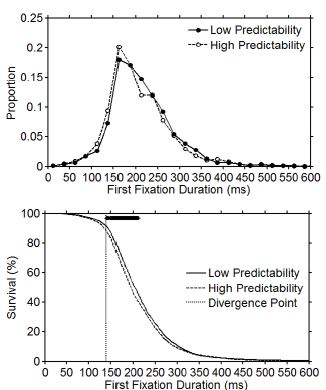
\includegraphics[width=2.4in]{heather1.jpg} 
    			\label{fig:dvff}
 		\end{figure}		
	}

	\frame
	{
		\frametitle{Divergence point}
		\begin{itemize}
			\item Clearly, if this method works there could be many applications for it.
			\item Sheridan and cols have presented analyses of eye movement data using this method.
		\end{itemize}
	}
	
}


\section{Flaws}
{

	\frame
	{
		\frametitle{Let's cut to the chase}
		Estimating divergence points in latency distributions is conceptually flawed.
	}
	
	\frame
	{
		\frametitle{Assumption}
			The two conditions share a process, and this is followed by a subsequent processing component in which the two conditions differ (diverge) on the timing and/or the processing cost.
	}
	
	\frame{
	\frametitle{Realistic assumption?}
		Although one could think of somewhat contrived situations in which this type of serial, staged process might occur (see Carreiras, Armstrong, Perea, \& Frost, 2014, for a recent review against this type of formulation), the latencies, even at their shortest duration, would  be a reflection of the \textbf{ending times} of the second process. 
	}
	
	\frame{
	\frametitle{In short}
	Latency distributions reflect aggregation across processes, across trials, and even across participants. 
	}

        \frame{
        \frametitle{How do we know this?}
        		Latency measurements show stochastic dominance.
        }
        
        \frame{
        \frametitle{Stochastic dominance}
        
        Stochastic dominance refers to the probability of observations smaller than x being greater for one variable than the other for all values of x (see Heathcote, Brown, Wagenmakers, \& Eidels, 2010).
        }
        
        
        \frame{
        \frametitle{Example,cumulative density functions generated with an ex-Gaussian distribution in which there are effects on $\mu$}
        
       \begin{figure}[p] %  figure placement: here, top, bottom, or page
	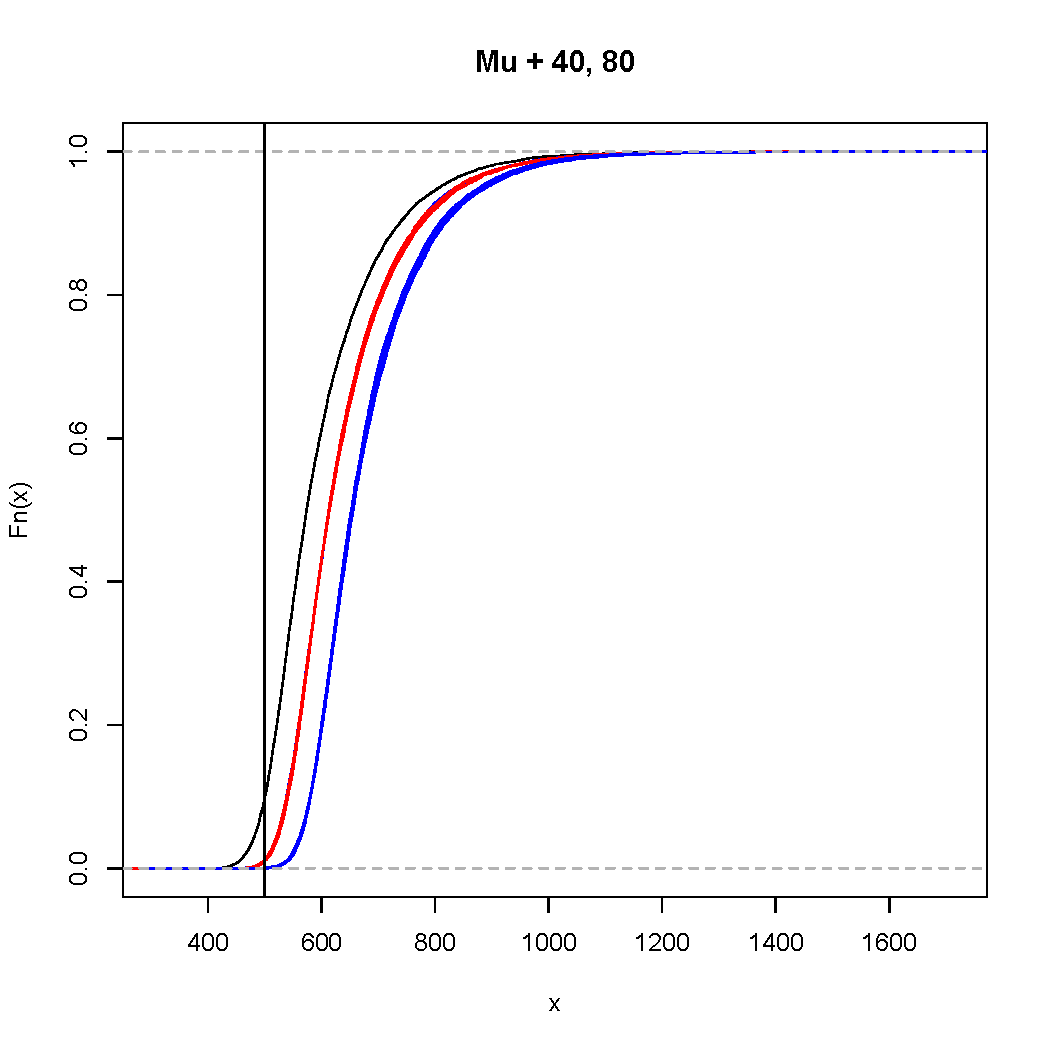
\includegraphics[width=3in]{Figure2.pdf}
   	\label{fig:mu}
\end{figure}		
}


        \frame{
        \frametitle{Example,cumulative density functions generated with an ex-Gaussian distribution in which there are effects on $\tau$}
        
       \begin{figure}[p] %  figure placement: here, top, bottom, or page
	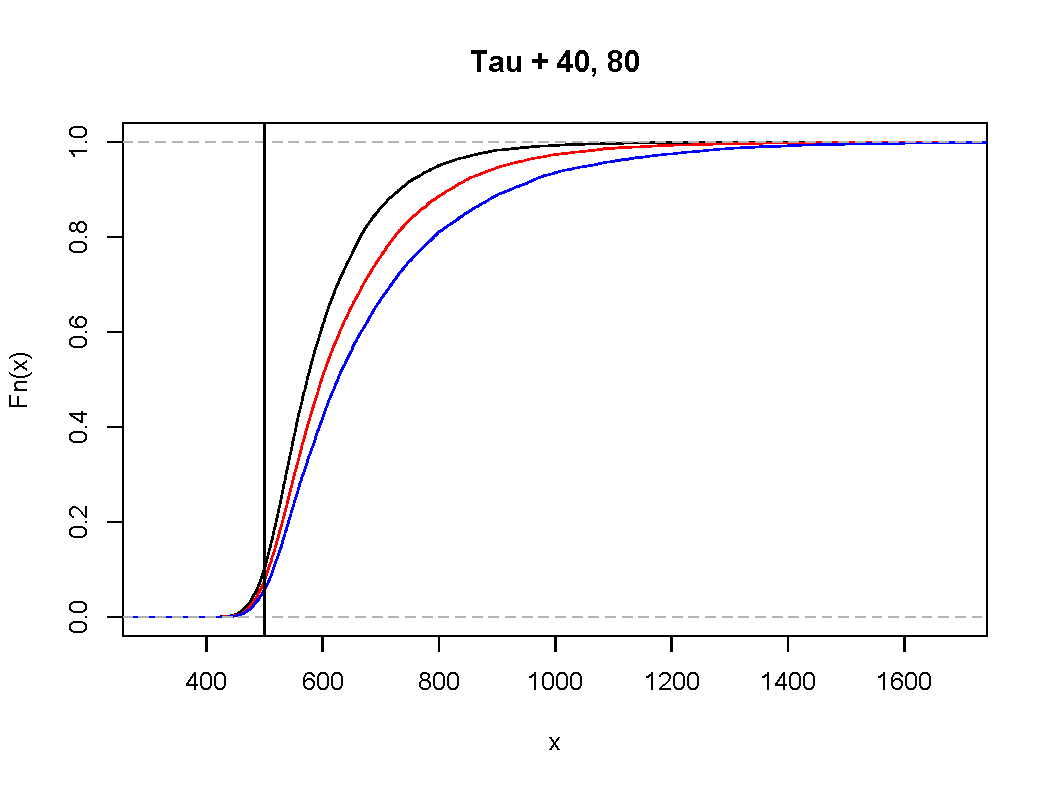
\includegraphics[width=3in]{Figure3.pdf}
   	\label{fig:mu}
\end{figure}		
}


}       
  




\section{Simulation studies}
{
	\frame
	{
		\frametitle{Rationale}
		What are the consequences of applying this method to data in which there is stochastic dominance?
		\begin{itemize}
			\item Generate data from an ex-gaussian distribution assuming that the experimental effect is either in the $\mu$ or $\tau$ parameters of the ex-gaussian.
			\item Create latencies manipulating the number of hypothetical trials per condition.			
			\item We apply the bootstrapping method.
			\item We explore if the method recovers the properties of the data generating strategy.
		\end{itemize}
	}
	
	
	\frame
	{
		\frametitle{Effects on $\mu$}
			\begin{itemize}
				\item Data generated from an ex-gaussian with $\mu= 541$; $\sigma = 68$; $\tau = 115$; $\Delta_\mu = 20$, 40, 80.
				\item Shift in distribution.... in other words, stochastic dominance, divergence happens at shortest latencies!
			\end{itemize}
	}	
	\frame
	{
			
		\frametitle{Effects on $\mu$}
		A biased estimation of divergence point
		\begin{figure}[htbp] %  figure placement: here, top, bottom, or page
    			\centering
    			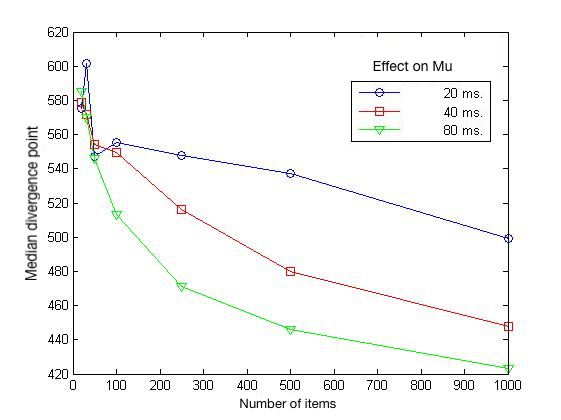
\includegraphics[width=2.4in]{mu-all.jpg} 
    			\label{fig:dvff}
 		\end{figure}		
	
	}
	
	
	\frame
	{
		\frametitle{Effects on $\tau$ with large $\tau$ values}
			\begin{itemize}
				\item Data generated from an ex-gaussian with  $\mu= 541$; $\sigma = 68$; $\tau = 115$; $\Delta_\tau = 20$, 40, 80.
				\item Change in tail... in other words, stochastic dominance, divergence happens at shortest latencies!

			\end{itemize}
	}	
	\frame
	{
			
		\frametitle{Effects on $\tau$ with large $\tau$ values}
		A biased estimation of divergence point
		\begin{figure}[htbp] %  figure placement: here, top, bottom, or page
    			\centering
    			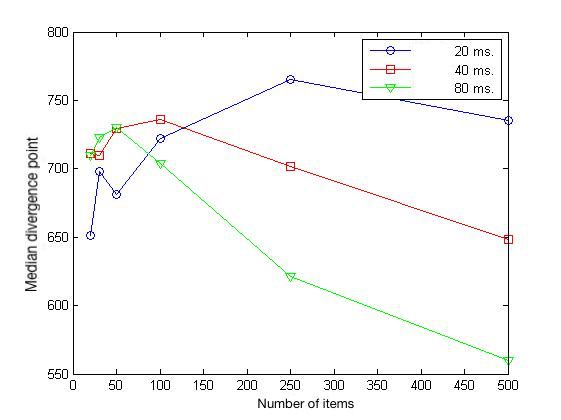
\includegraphics[width=2.4in]{tau-all.jpg} 
    			\label{fig:dvff}
 		\end{figure}		
	
	}
	
	\frame
	{
		\frametitle{Effects on $\tau$ with small $\tau$ values}
			\begin{itemize}
				\item Data generated from an ex-gaussian with  $\mu= 541$; $\sigma = 68$; $\tau = 20$; $\Delta_\tau = 20$, 40, 80.
				\item Change in tail : The method should give us a divergence point later on.
			\end{itemize}
	}	
	\frame
	{
			
		\frametitle{Effects on $\tau$ with small $\tau$ values}
		A biased estimation of divergence point
		\begin{figure}[htbp] %  figure placement: here, top, bottom, or page
    			\centering
    			\includegraphics[width=2.4in]{tau2-all.jpg} 
    			\label{fig:dvff}
 		\end{figure}		
	
	}
	
	
	
	
	
	
	\frame
	{
		\frametitle{Summary of results}
			\begin{itemize}
				\item With number of items within the standard cognitive psychology experiment, the method severely overestimates the point in time of the divergence.
				\item As it stands, the method provides with an output  that is mostly related to the number of items per condition.  
			\end{itemize}
		

	}
}	
\section{Conclusion}
{

	\frame
	{
	\frametitle{Take home message (I)}

Latency measurements tend to exhibit stochastic dominance between experimental conditions, and hence the divergence point would be at the leading edge of the latency distribution regardless of other distributional differences.
}


	\frame
	{

		\frametitle{Take home message (II)}

  Furthermore, if the method is applied to data, an estimate of the divergence point will be provided by the method. This estimate will be affected heavily by the number of observations.   In short, our exploration of the method forces us to conclude that it is not advisable to utilize it when analyzing latency data.

	
	
	}			
	
	
	\frame{	
		Thank you!
	}		
}

\end{document}
